\documentclass[11pt]{article}
\usepackage[margin=1in]{geometry}
\usepackage{graphicx}
\usepackage{amsmath}
\usepackage{booktabs}
\title{A Finite Intercept Correction Calculation}
\author{Anonymous}
\date{}
\begin{document}
\maketitle
\begin{abstract}
This anonymous synthetic teaching-note workflow demonstration examines an additive correction to the fixed predictor $2x$ on five observations with targets $y=2x+3$. The mean observed residual gives $b=3$, making corrected predictions $2x+b$ equal the supplied targets. Recorded mean absolute error decreases from $3$ to $0$, and mean squared error from $9$ to $0$. A measured error table and two reproducible figures expose the computation. Correction and evaluation reuse the same observations; the results establish finite arithmetic agreement without predictive generalization or methodological novelty.
\end{abstract}
\section{Introduction}

Residuals make discrepancies between observations and predictions explicit, and their examination has a substantial methodological history \cite{Anscombe1963ExaminationAnalysis,Denby1987ExampleUse,Chatterjee1986InfluentialObservations,Cook1977DetectionInfluential}. This teaching note uses a completely specified example to explain a constant prediction discrepancy, its correction, and the interpretation of the resulting errors.

The supplied observations are
\[
x=(-2,-1,0,1,2), \qquad y=(-1,1,3,5,7),
\]
with $y_i=2x_i+3$ on these five points. The baseline predictor $f_0(x)=2x$ leaves residual $3$ at every observation, so their mean gives
\[
b=\frac{1}{5}\sum_{i=1}^{5}(y_i-2x_i)=3.
\]
Adding this value reproduces all five targets. The recorded mean absolute errors at $b=0,1.5,3$ are $3,1.5,0$, and the mean squared errors are $9,2.25,0$.

These numbers describe the observations used to determine the correction. Distinguishing descriptive or explanatory success from predictive performance is a broader concern \cite{Shmueli2010ExplainOr,Yarkoni2017ChoosingPrediction}, and reusing fitting data can produce optimistic assessments \cite{Efron1986HowBiased,Efron2004EstimationPrediction}. Our objective is an inspectable arithmetic demonstration, not a new algorithm or scientific result. The calculation contains no stochastic repetitions or held-out evaluation; its zero recorded errors establish exact agreement on the five supplied points only.

\section{Related Work}

\subsection{Additive Correction of a Fixed Predictor}

Regression without an intercept raises known questions about when origin constraints are appropriate \cite{Hahn1977FittingRegression,Eisenhauer2003RegressionThrough}. In the present example, however, the slope is supplied as $2$ and never estimated; the calculation changes only the constant term.

Post-processing methods also adjust predictors after construction. Sigmoid fitting produces probabilities from support-vector-machine outputs \cite{Platt1999ProbabilisticOutputs}, temperature scaling adjusts classification confidence \cite{Guo2017CalibrationModern}, and calibrated regression addresses predictive uncertainty \cite{Kuleshov2018AccurateUncertainties}. Our response-scale addition neither estimates class probabilities nor calibrates uncertainty. Intercept recalibration has also been studied in clinical validation \cite{Steyerberg2004ValidationUpdating}, but those findings do not transfer to five synthetic observations.

\subsection{Error Summaries and Reuse of Fitting Observations}

Point-forecast evaluation depends on matching the scoring function to the task \cite{Gneiting2011MakingEvaluating}, and the relative merits of MAE and RMSE have been debated \cite{Willmott2005AdvantagesMean,Hodson2022RootmeansquareError}. For each recorded correction, all five residuals equal $3-b$, so the reported MAE and MSE are $|3-b|$ and $(3-b)^2$. The log reports MSE, whereas much of the cited metric discussion concerns its square root, RMSE.

Reusing data for both tuning and assessment can bias error estimates \cite{Varma2006BiasError}. Our calculation performs neither model selection nor cross-validation. Here, the same five targets determine $b$ and evaluate $2x+b$; no held-out accuracy, uncertainty estimate, or statistical significance is established.

\section{Method}

\subsection{Finite Calculation and Error Definitions}

Index the supplied inputs by $i=1,\ldots,5$, with targets $y_i=2x_i+3$. The fixed baseline predictions are
\[
\hat{y}^{(0)}=(-4,-2,0,2,4),
\]
with observed residuals
\[
r_i=y_i-\hat{y}^{(0)}_i=3,
\qquad r=(3,3,3,3,3).
\]
For an added scalar $b$, define $\hat{y}_i(b)=2x_i+b$ and $e_i(b)=y_i-\hat{y}_i(b)$. The two error summaries are
\[
\operatorname{MAE}(b)=\frac{1}{5}\sum_{i=1}^{5}|e_i(b)|,
\qquad
\operatorname{MSE}(b)=\frac{1}{5}\sum_{i=1}^{5}e_i(b)^2.
\]
Substitution gives $e_i(b)=3-b$ on every supplied observation, hence
\[
\operatorname{MAE}(b)=|3-b|,
\qquad
\operatorname{MSE}(b)=(3-b)^2.
\]
These finite identities explain the recorded settings; they are not measurements at additional settings.

\subsection{Mean Residual Correction and Computational Flow}

The correction is computed directly:
\[
b=\frac{1}{5}\sum_{i=1}^{5}r_i
=\frac{3+3+3+3+3}{5}=3.
\]
Consequently, $\hat{y}(3)=(-1,1,3,5,7)=y$, so each corrected residual is zero. The calculation uses base R, with no optimizer or iterative training procedure.

Figure~\ref{fig:residual_workflow} shows the dependencies: targets and baseline predictions determine residuals, whose mean determines the correction. The dashed path discloses reuse of the original observations for evaluation. The schematic explains this computation and supplies no additional empirical evidence.

\begin{figure}[htbp]
    \centering
    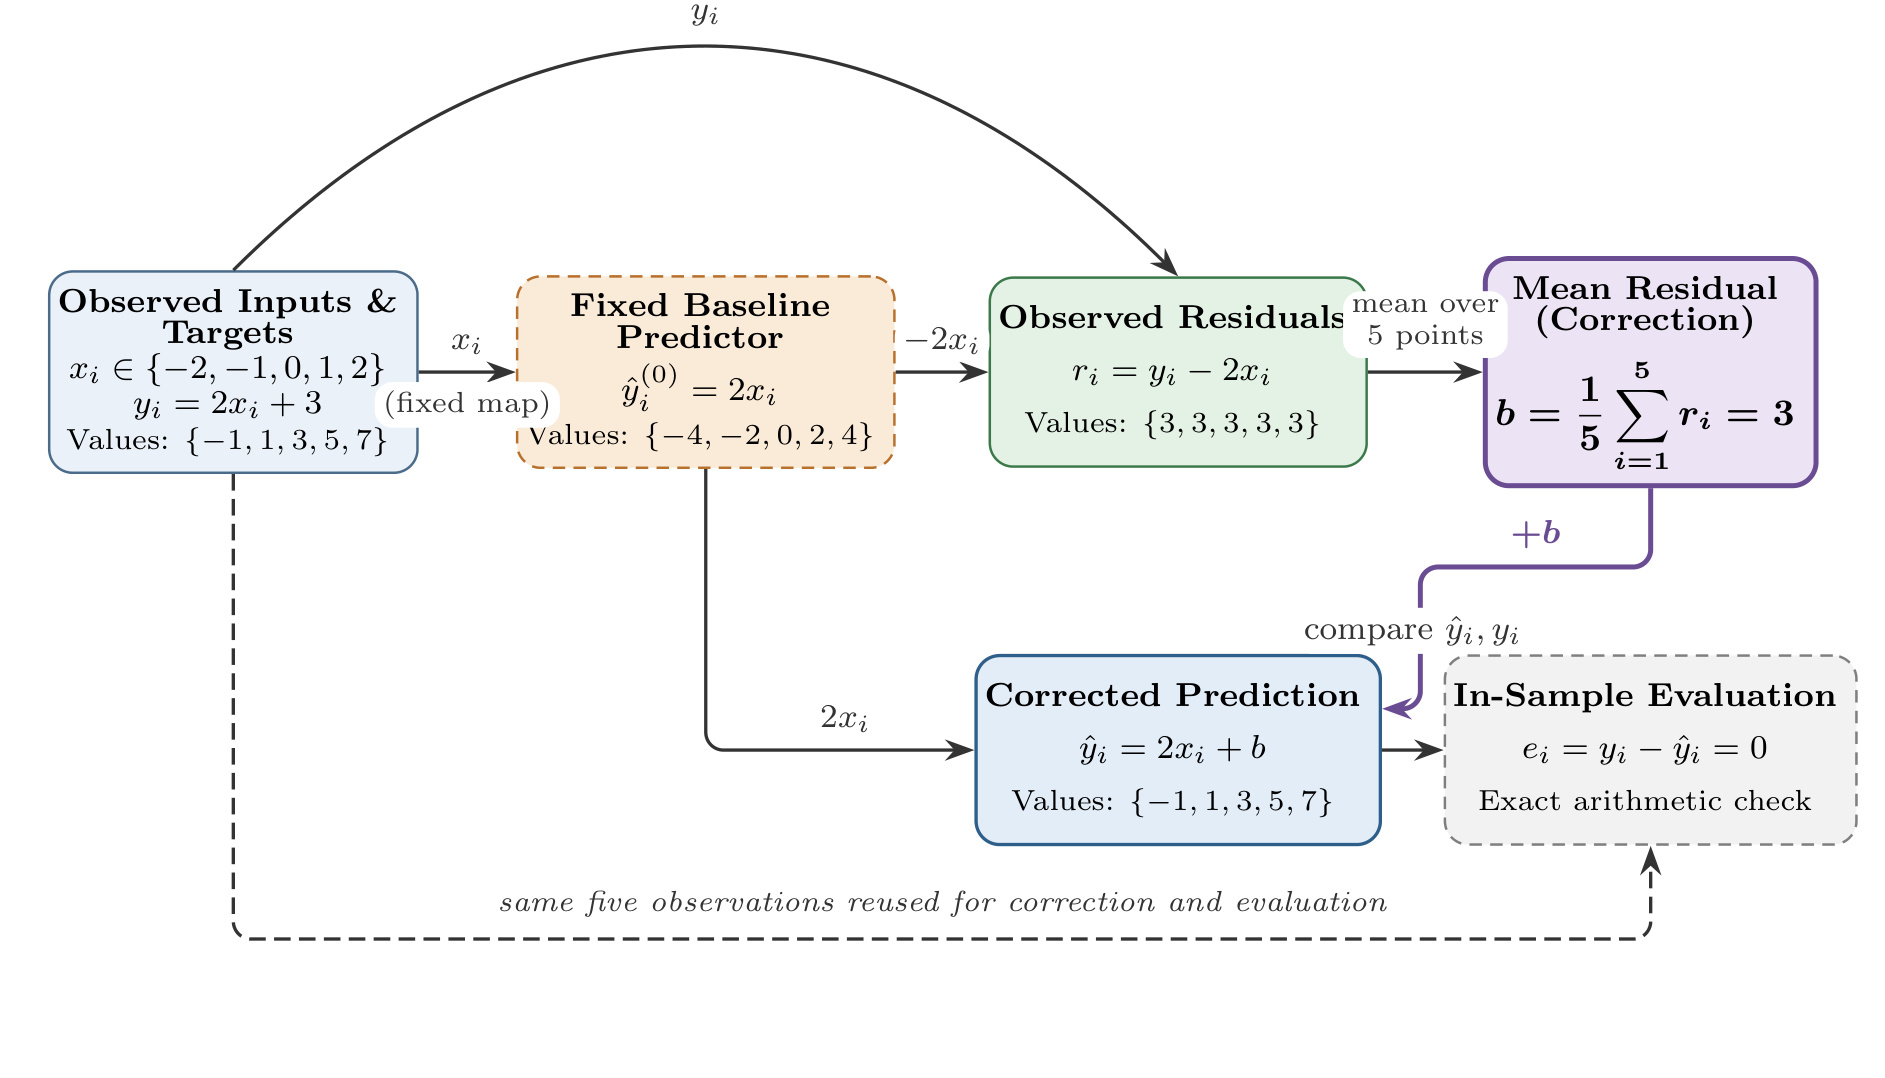
\includegraphics[width=\linewidth]{figures/fig_residual_workflow.jpg}
    \caption{Residual-based intercept correction on five synthetic observations. Observed targets and fixed baseline predictions determine residuals $r_i=y_i-2x_i=3$; their mean determines $b=3$. Adding $b$ reproduces the targets. The dashed path identifies reuse of the same five observations for correction and in-sample evaluation.}
    \label{fig:residual_workflow}
\end{figure}

\section{Experiments}

\subsection{Observations and Evaluation Protocol}

The experimental log records one deterministic calculation on supplied synthetic values rather than a named external dataset. Targets are $(-1,1,3,5,7)$, baseline predictions are $(-4,-2,0,2,4)$, and predictions after adding $3$ are $(-1,1,3,5,7)$. The three settings $b=0,1.5,3$ are controlled changes to one scalar within the same calculation, not independent experiments. The slope remains fixed throughout. There is no held-out evaluation, timing measurement, optimizer training, architecture comparison, or uncertainty estimate.

\subsection{Recorded Errors and Reproducible Figures}

Table~\ref{tab:recorded_errors} reproduces the logged measurements. The uncorrected setting retains the entire constant discrepancy. Adding $1.5$ removes half of it: MAE falls from $3$ to $1.5$, and MSE falls from $9$ to $2.25$. Adding the full mean residual, $3$, removes it entirely. Because every residual has the same magnitude at each setting, the different reductions follow from absolute versus squared error aggregation.

\begin{table}[htbp]
    \centering
    \caption{Recorded errors on the same five observations used to determine the correction.}
    \label{tab:recorded_errors}
    \begin{tabular}{rrr}
        \toprule
        Added $b$ & Mean absolute error & Mean squared error \\
        \midrule
        0   & 3   & 9    \\
        1.5 & 1.5 & 2.25 \\
        3   & 0   & 0    \\
        \bottomrule
    \end{tabular}
\end{table}

Figure~\ref{fig:intercept_error} displays exactly these three recorded MSE values, without an interpolated curve or uncertainty intervals. The scalar adjustment succeeds here because the observed discrepancy is constant. No supplied result tests correction of a nonconstant residual pattern, so independent observations and other patterns remain subjects for future evaluation.

\begin{figure}[t]
    \centering
    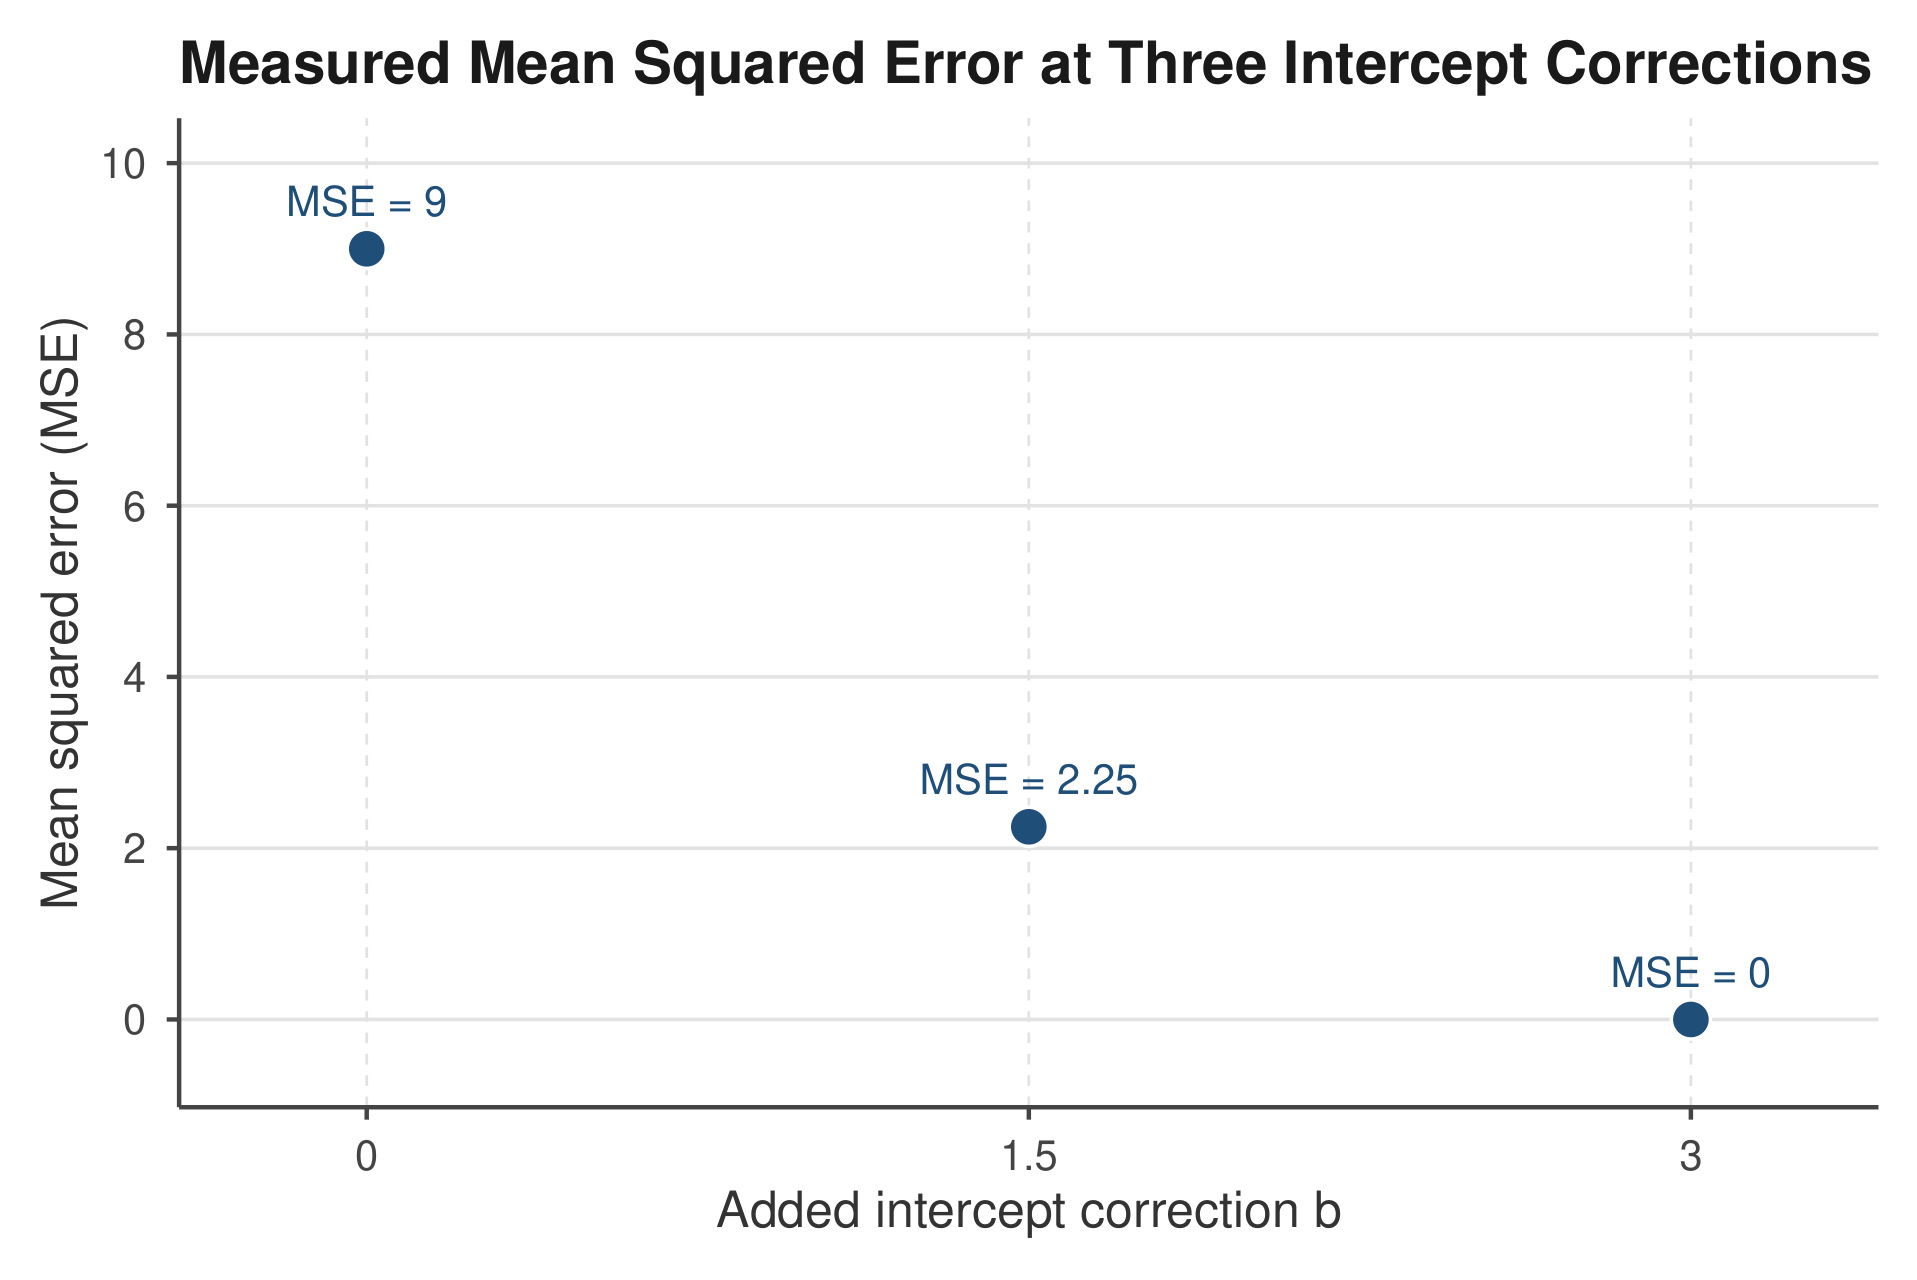
\includegraphics[width=\linewidth]{figures/fig_intercept_error.jpg}
    \caption{Exactly three recorded mean squared errors: $(b,\operatorname{MSE})=(0,9),(1.5,2.25),(3,0)$. Evaluation uses the same five synthetic observations that determine $b=3$. The points establish finite arithmetic error reduction only.}
    \label{fig:intercept_error}
\end{figure}

\section*{Figure source provenance}

The supplied figure images are used unchanged. The selected editable R/ggplot2 source for Figure~\ref{fig:intercept_error} is
\[
\text{\texttt{\detokenize{figure_code/fig_intercept_error/source.R}}}.
\]
Its rendering worker is
\[
\text{\texttt{\detokenize{figure_code/fig_intercept_error/worker.R}}}.
\]
The selected editable LaTeX/TikZ source for Figure~\ref{fig:residual_workflow} is
\[
\text{\texttt{\detokenize{figure_code/fig_residual_workflow/source.tex}}}.
\]
These sources are separate reproducibility artifacts, and the figure recipes are not reconstructed or embedded in the manuscript.

\section{Conclusion}

The mean observed residual $b=3$ makes $2x+b$ equal all five supplied targets, reducing recorded MAE and MSE to zero. The explicit calculation, measured error table, and two reproducible figures support an inspectable teaching-note demonstration. Correction and evaluation reuse the same five observations. The note consequently supplies no held-out performance or generalization result; assessment on independent observations remains future work.

\bibliographystyle{plain}
\bibliography{references}

% PAPER_ORCHESTRA_PROVENANCE_BEGIN
\clearpage
\section*{Figure source provenance}
The files below are the exact sources that produced the embedded figure previews. Paths are relative to this manuscript's source directory. The accompanying \texttt{figure\char95{}provenance.json} records all artifact checksums.\par
\medskip\noindent\textbf{Figure~\ref{fig:intercept_error} (\texttt{fig\char95{}intercept\char95{}error.jpg}).}\par
\noindent R/ggplot2 source: \texttt{figure\char95{}code/\allowbreak{}fig\char95{}intercept\char95{}error/\allowbreak{}source.R}.\par
\noindent Source SHA256: \texttt{2479e40e\allowbreak{}8d39e8e1\allowbreak{}6c29f883\allowbreak{}7e3b8df9\allowbreak{}909f9f65\allowbreak{}8bb35b95\allowbreak{}9fda0b12\allowbreak{}96debbe4}.\par
\noindent Rendering metadata: \texttt{figure\char95{}code/\allowbreak{}fig\char95{}intercept\char95{}error/\allowbreak{}render.json}.\par
\noindent Exact export wrapper: \texttt{figure\char95{}code/\allowbreak{}fig\char95{}intercept\char95{}error/\allowbreak{}worker.R}.\par
\noindent Wrapper SHA256: \texttt{1aedad4b\allowbreak{}1547d4b2\allowbreak{}d394cbb0\allowbreak{}239655d3\allowbreak{}667d453d\allowbreak{}d1fd0eca\allowbreak{}3e77c037\allowbreak{}e6d34892}.\par
\noindent Rendering metadata: \texttt{figure\char95{}code/\allowbreak{}fig\char95{}intercept\char95{}error/\allowbreak{}sessionInfo.txt}.\par
\medskip\noindent\textbf{Figure~\ref{fig:residual_workflow} (\texttt{fig\char95{}residual\char95{}workflow.jpg}).}\par
\noindent LaTeX/TikZ source: \texttt{figure\char95{}code/\allowbreak{}fig\char95{}residual\char95{}workflow/\allowbreak{}source.tex}.\par
\noindent Source SHA256: \texttt{84e305cc\allowbreak{}09efdeb2\allowbreak{}bc2162c3\allowbreak{}9fc60cb1\allowbreak{}d1a3c538\allowbreak{}4254d368\allowbreak{}dee04e8d\allowbreak{}b66664b4}.\par
\noindent Rendering metadata: \texttt{figure\char95{}code/\allowbreak{}fig\char95{}residual\char95{}workflow/\allowbreak{}render.json}.\par
% PAPER_ORCHESTRA_PROVENANCE_END
\end{document}